\chapter{Conception de la Base de Données}

La conception de la base de données est au cœur de notre application. Pour garantir l'intégrité des données des salles, du personnel et du matériel, nous avons choisi une modélisation relationnelle sous PostgreSQL. Les tables utilisent des identifiants UUID pour garantir l'unicité des données ; les coordonnées des salles sont stockées au format JSONB afin de conserver une représentation structurée et extensible des positions et dimensions des zones sur les plans.

\section{Modèle Logique de Données (MLD)}
Le schéma ci-dessous présente l'organisation des tables et les relations entre elles. Il met l'accent sur les contraintes d'intégrité référentielle (clés primaires et étrangères), qui assurent la cohérence des informations de l'inventaire et de l'occupation des salles.

\begin{figure}[h]
    \centering
    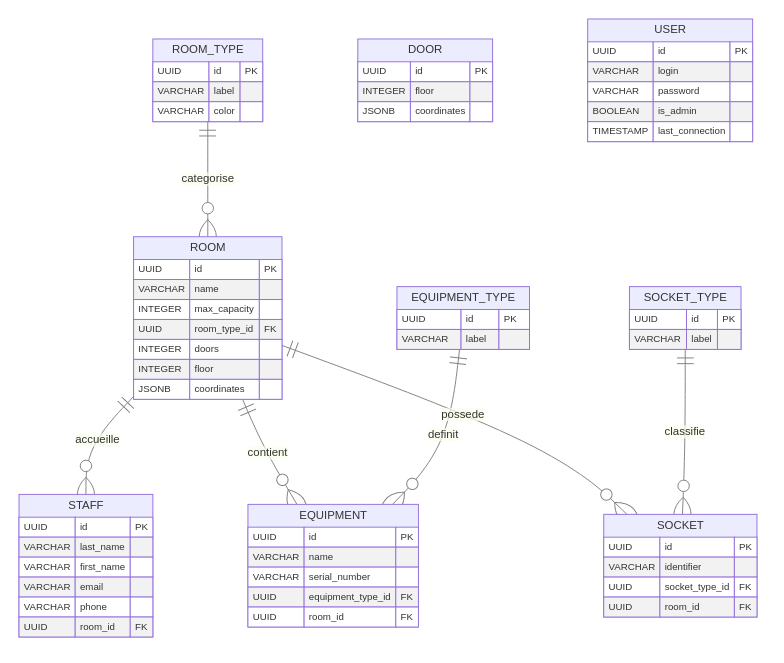
\includegraphics[width=0.7\textwidth]{img/schema_db.png}
    \caption{Schéma relationnel de la base de données PostgreSQL}
    \label{fig:mld_db}
\end{figure}

\section{Détail des tables et contraintes}
\begin{itemize}
    \item \textbf{Table \texttt{room}} : Elle modélise les espaces physiques. Chaque salle est caractérisée par sa capacité maximale, son type, son étage et ses coordonnées pour le plan.
    \item \textbf{Table \texttt{staff}} : Elle contient le personnel affecté aux locaux. La relation \texttt{room\_id} permet de savoir où chaque employé est positionné.
    \item \textbf{Table \texttt{user}} : Cette table stocke les comptes d'accès à l'application, ainsi que les informations de profil. Le champ \texttt{is\_admin} distingue les utilisateurs avec droits d'administration des utilisateurs standards.
    \item \textbf{Tables de référence} : \texttt{room\_type}, \texttt{equipment\_type} et \texttt{socket\_type} garantissent la cohérence des catégories utilisées dans les salles, le matériel et les prises.
    \item \textbf{Table \texttt{room\_type}} : contient le label et un champ \texttt{color} (couleur hexadécimale) utilisé par le frontend pour coloriser les salles dans les listes.
    \item \textbf{Table \texttt{equipment}} : Elle représente l'inventaire matériel d'une salle. Chaque équipement est lié à un type et peut être rattaché à une salle.
    \item \textbf{Table \texttt{socket}} : Elle répertorie les prises présentes dans chaque salle et les associe à un type de connectique.
    \item \textbf{Table \texttt{door}} : Elle modélise les points d'accès (portes) sur les plans, avec leur étage et leurs coordonnées stockées en \texttt{JSONB}.
\end{itemize}

Le schéma présenté regroupe donc les tables principales suivantes : \texttt{room}, \texttt{door}, \texttt{staff}, \texttt{equipment}, \texttt{socket}, ainsi que les tables de référence \texttt{room\_type}, \texttt{equipment\_type}, \texttt{socket\_type} et la table \texttt{user} pour la gestion des accès.

La modélisation adopte des règles solides : les types de référence sont supprimés en cascade, tandis que les dépendances sur les salles sont gérées avec \texttt{SET NULL} lorsque cela est pertinent, afin de préserver les données historiques et limiter les pertes involontaires.